\chapter{The Proposed Method} \label{proposmeth} 
In this chapter, an architecture for developing interactive learning environments is proposed. The architecture allows the use of techniques of adaptive hypermedia systems and use in interactive environments. This architecture has as resources environmental learning objects, which are presented to users through the various devices that can be part of this environment and are organized by a sequence based on Simple Sequencing. Also a new method to automate the measurement of the level of attention of the user without using invasive methods. In Figure \ref{arquitectura} we can observe the components of this architecture. As this environment has multiple configurations of use, sometimes it can help a fuzzy inference system to adapt the information presented by the environment to users. The components of the architecture are described in detail.

\begin{figure}[ht!]  
\centering  
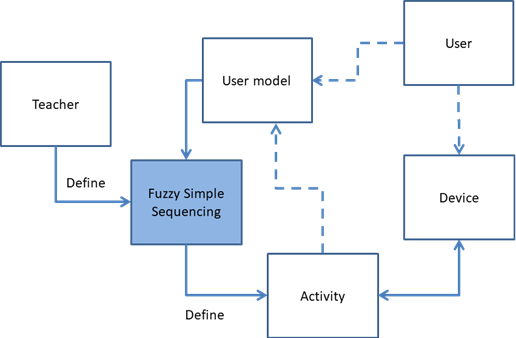
\includegraphics[scale=1]{arquitectura}
\quad  
\caption{Adaptive Learning Environment Architecture}  
\label{architecture}  
\end{figure}


\section{Environment}
%Los ambientes inteligentes son espacios con sistemas embebidos, sensores y tecnolog�as de informaci�n y comunicaci�n que se van haciendo imperceptibles para el usuario a media que van siendo integrados en objetos f�sicos, infraestructuras, el entorno en que vivimos, el trabajo y muchos otros ambientes. Los ambientes inteligentes interactivos facilitan herramientas con las cuales los usuarios pueden interactuar, lo que hace que este espacio sea interactivo por lo que la computaci�n se aproxima m�s al usuario. Existen otros tipos de ambientes como e-learning que son ambientes de aprendizaje virtuales donde un usuario aprende individualmente ciertos temas a partir de objetos de aprendizaje. Los trabajos en este tipo de ambientes de aprendizaje han utilizado diferentes t�cnicas para secuenciar y seleccionar los objetos de aprendizaje para cubrir las necesidades de aprendizaje del individuo como el secuenciado simple (referencia a la tesis del profe). 

Intelligent environments are spaces with embedded systems, sensors and information and communication technologies that are becoming imperceptible to the average user that are being integrated into physical objects, infrastructures, the environment in which we live, work and many other environments.
Intelligent interactive environments provide tools with which users can interact, which makes this space interactive so that the computer is closer to the user. There are other types of environments such as e-learning that are virtual learning environments where a user learns individually certain topics from learning objects. The work in this type of learning environments has used different techniques to sequence and select learning objects to cover the learning needs of the individual such as simple sequencing (referencia a la tesis del profe). 

\begin{figure}[ht!]  
\centering  

\includegraphics[scale=1]{elearning}
\quad  
\caption{E-Learning}  
\label{keyvalue}  
\end{figure}
The problem we notice is that most of them focus on a single solution, either oriented to learning, modify the environment, that handle only one user at a time. In reviewing the literature we realized that by combining certain standards there is an improvement in the user's learning experience. Currently there are certain limitations with intelligent environments such as:
\begin{itemize}	
\item Learning environments are designed so that learning objects are used by one user at a time.
\item Contextual information is sometimes not considered.
\item Usually the environment can not be taken to other places without having to make modifications.
\item Some works with environments use devices that are not as advanced as they are now, and have become more accessible economically.
\end{itemize}

%Proponemos generar un ambiente que gracias a un servicio web sea capaz de atacar todas las limitaciones que observamos en los ambientes de aprendizaje actuales. Gracias a los servicios web podemos crear repositorios que pueden estar disponibles siempre y cuando exista una conexion a internet, pero que pasa con aquellos lugares donde no exista tal conexion, para estos casos se puede llevar un repositorio que sirva como local para poder obtener los objetos de aprendizaje o el contenido. Ademas el ambiente esta centrado para atender a un grupo de usuarios.
We propose to generate an environment that thanks to a web service is capable of attacking all the limitations that we observe in the current learning environments. Thanks to the web services we can create repositories that can be available as long as there is an internet connection. But what about those places where there is no such connection? For these cases you can take a repository that serves as a local to be able to obtain learning objects or content. In addition the environment is focused to serve a group of users.

%El ambiente de aprendizaje propuesto tiene proyectados varios usos, el primero de ellos y obviamente como ambiente de aprendizaje, como exhibidor de museo, entrenamiento, entretenimiento, publicidad, juegos. y esto es posible gracias al servicio web que permite utilizar diferentes objetos de aprendizaje y de diferentes tipos en cualquier dispositivo sea capaz de correr un navegador web y que este disponible.
The proposed learning environment has several uses, the first of them and obviously as a learning environment, as a museum exhibitor, training, entertainment, advertising, games. And this is possible thanks to the web service that allows to use different learning objects and of different types in any device that is able to run a web browser and that it is available.
Then we will be concerned with the learning part, the modification of the environment and the user resulting in a learning environment that can be manipulated or adjusted to the needs of the users. In order to carry out this, we propose a new learning object methodology, which we will call "Environmental Learning Object", this object will be used in a learning environment where users can interact with it. We will speak more specifically about this proposal later.

\section{ELO}
A standard learning object is defined in \cite{wayneh}. The teacher prepares teaching materials using content from various sources; select different pieces of information that subsequently assembled to form the course or class to teach. Learning objects are based on this methodology, seeing the didactic content as a component that is designed to combine with others and to be used in different contexts; learning objects usually have the following characteristics: 
�	They are self-contained. Each learning object can be used independently. 
�	Are reusable. A learning object can be used in different contexts, for multiple purposes. 
�	Can be added. Learning objects can be grouped into collections, after being presented with a traditional course structure. 
�	Are labeled with metadata. Each learning object has associated certain in-formation that describes it. This facilitates reuse by automatic means.

\subection{Proposed learning object}
We propose a learning environment that uses a new type of learning object which we call "Environmental Learning Object" (ELO) these objects include additional metadata that can be used to identify and manage content for their use in ubiquitous devices: we considered input and output devices e.g. interactive tables, wall projections, monitors, tablets, cameras, microphones and speakers.
By tagging through the metadata we can make a selection of learning objects to create and manage different contexts when applied to a learning environment as we can note in Figure.
Where each learning object is selected and routed to a device that operates its utility like a sound file that can�t be used on a monitor maybe on a Smartphone or a tablet pc, these are the types of problems that can occur when using these learning objects. Also this ELO will give contextual information for feedback. 
\subection{Formal definition.}
Objeto de Aprendizaje Ambiental (OAA) es un objeto de aprendizaje que permite la distribuci�n de contenido a diversos dispositivos con la condici�n de que deben estar disponibles y ser compatibles en un ambiente de aprendizaje interactivo.
Un objeto de aprendizaje ambiental (OAA) se determina por la tupla <O,D> donde O es un conjunto de objetos de aprendizaje y D es un conjunto de Dispositivos.
OOA=((O,D),D)

Donde un objeto de aprendizaje o ? O objetos de aprendizaje como entidades, digitales o no digitales, que pueden ser utilizadas para promover el aprendizaje, educaci�n o entrenamiento.
Y un dispositivo d ? D dispositivos con la condici�n de que deben estar disponibles y ser compatibles en un ambiente de aprendizaje interactivo.

\subection{Formal definition.}
\section{Fuzzy simple sequencing}
Simple sequencing standard[18] [19], which allows sequencing of this type of learning objects. First an activity tree with n number of activities is determined by the teacher, selecting the learning objects to be used per activity and adding fuzzy pre-condition rules that consider the context and user model to determine the sequence, for example:
IF Context.Temperature is HIGH and Session.Activity.Place is OUTSIDE
THEN
this.Precondition. = SKIP.
Then context information is obtained from users using the sensors mentioned above, each activity will have 1 or more environmental learning objects, thanks to the metadata included in the learning objects will be displayed in the appropriate device for example if we have a web page can be displayed on a monitor, a questionnaire on a tablet, a video projected on a wall, sound on speakers, an interactive game on the table as we can see in Figure 3.
The main components of the Simple Sequencing standard are the Learning Activities and the Activity Tree. A Learning Activity is defined as a pedagogically neutral unit of instruction, knowledge, evaluation, etc. Learning Activities can have nested sub-activities arbitrary depth. 
There is an implicit hierarchy of containers in the tree. Depending on the application concept labels can be applied to learning activities. Only leaf nodes can be associated with Resources Activity (the equivalent of Learning Objects).An example of the configuration obtained by sequencing can be observed in Figure 3.2. The tree is traversed as follows from the root there is the General activity (can be any subject in particular) with 2 nodes in it, we see that has the attribute "forwardOnly" on true, this means they have to be traveled sequentially by users, the first activity is a pre-evaluation, which is associated with a learning object in this case a test that contains a rule that makes the activity is carried out or otherwise will not advance to the next activity, as specified in the Pre\_condition rule.
When a learning sequence is generated learning activities are established and they not change, what changes is the action as if you skip, performed, jump, hide, repeat or show an activity, this decision is taken by the rules of precondition. In this paper we seek to generate diversity of resources displayed in the activities adapting the resources of the activity to the user,  for example we have an introductory activity of a particular subject and 2 users of different ages perform the activity, the first user of 25 years will be shown more detailed and textual information, while the second user of 6 years of age is in a very early stage of learning resources that show you are easier to understand and have more audio-visual con-tent. With fuzzy logic generate inputs for use in the precondition rules for example: fuzzy rule if user.age is low and user.academic\_level is low then user.level is begginer. On the precondition rule we will use the output of the fuzzy rule will use the output of that fuzzy rule as follows if user=begginer then pre\_condition = show. Thus a set of resources is obtained for a novice user and these are shown on the right devices for each resource through a web browser running in this device as we can see on the figure 1.

\section{Devices}
\section{Master / User}
\section{Engagement}
The other way to obtain user information was by Kinect Sensor and is a bit more complex because the sensor provides enough information the sensor detects a user can give: 
� engage 
� looking away 
� happy 
� left eye closed 
� right eye closed
� mouth open 
� mouth moved 
� wearing glasses 
� yaw pitch and roll of the face
Each of these data the sensor assigned one of the following Yes, No, Maybe and Unknown values; unknown data were discarded since in the sensor documentation was saying that this data could be�not sensing� and therefore not considered valid data. Only in the face position was a numerical data, the sensor generated an average of 14 records per second of these values sometimes less for a short time when the sensor lost sight of the user but was usually between 1 to 10 seconds.
Full activity was carried out in 4 minutes 10 seconds so if the sensor not loses sight of the user throughout the activity it generates about 3500 records. From the above list of data we decided to use only engage, looking away happy and others are captured but used as they are not relevant to what we are measuring. To get textual results perform a normalization by a count of each event every 10 seconds since the data generated by the sensor are textual normalized by assigning numbers to strings for example Yes = 2, Maybe = 1 and No = 0 then for every 10 seconds of activity the Yes, No and Maybe was counted.
As the activity lasted 4:10 we decided to count the sensor event every 10 seconds, at the end we gained an average of 140 records for each period of 10 seconds. Here I was a problem, as the number of records varied by user we had to think about how to normalize this data, as records were recorded and distributed yes, maybe, no the solution was to take a percentage of each of the records obtained by which thus we could handle and sensor data.